\chapter{Titratie}\label{ch:g11:titration}

Op het doosje van een ijzersupplement staat dat elke tablet \qty{80}{mg}
ijzer bevat, als ijzer(II)\omterm{def:g9:ions:ion}{ionen}. Klopt dat? Een scheikundige verpulvert
een tablet, lost die op in zuur, en voegt druppel voor druppel een paarse
oplossing van kaliumpermanganaat toe uit een lange buis met een
maatverdeling. Elke druppel verliest meteen zijn kleur, omdat de
permanganaationen door de ijzer(II)\omterm{def:g9:ions:ion}{ionen} verbruikt worden, tot één
druppel, de laatste, een zwakke roze kleur achterlaat die niet meer
verdwijnt. Het volume dat op dat moment is toegevoegd, geeft de
hoeveelheid ijzer. Dit hoofdstuk maakt van een reactie een meting.

\begin{recall}
Een \omterm{def:g11:redox:oxidant}{oxidator} neemt \omterm{def:g9:inside-the-atom:nucleus}{elektronen} op, een \omterm{def:g11:redox:oxidant}{reductor} staat ze af; het
permanganaation oxideert ijzer(II)\omterm{def:g9:ions:ion}{ionen} volgens
\ce{MnO4^- + 8H+ + 5Fe^{2+} -> Mn^{2+} + 5Fe^{3+} + 4H2O}
(\cref{ch:g11:redox}). \omterm{def:g10:concentration-and-dilution:molar-concentration}{Molaire concentratie} en \omterm{def:g10:concentration-and-dilution:dilution}{verdunning}
(\cref{ch:g10:concentration-and-dilution}); de \omterm{def:g10:reaction-progress-table:extent}{voortgangstabel} en de
\omterm{def:g10:reaction-progress-table:limiting}{beperkende beginstof} (\cref{ch:g10:reaction-progress-table}).
\end{recall}

\begin{omfigure}
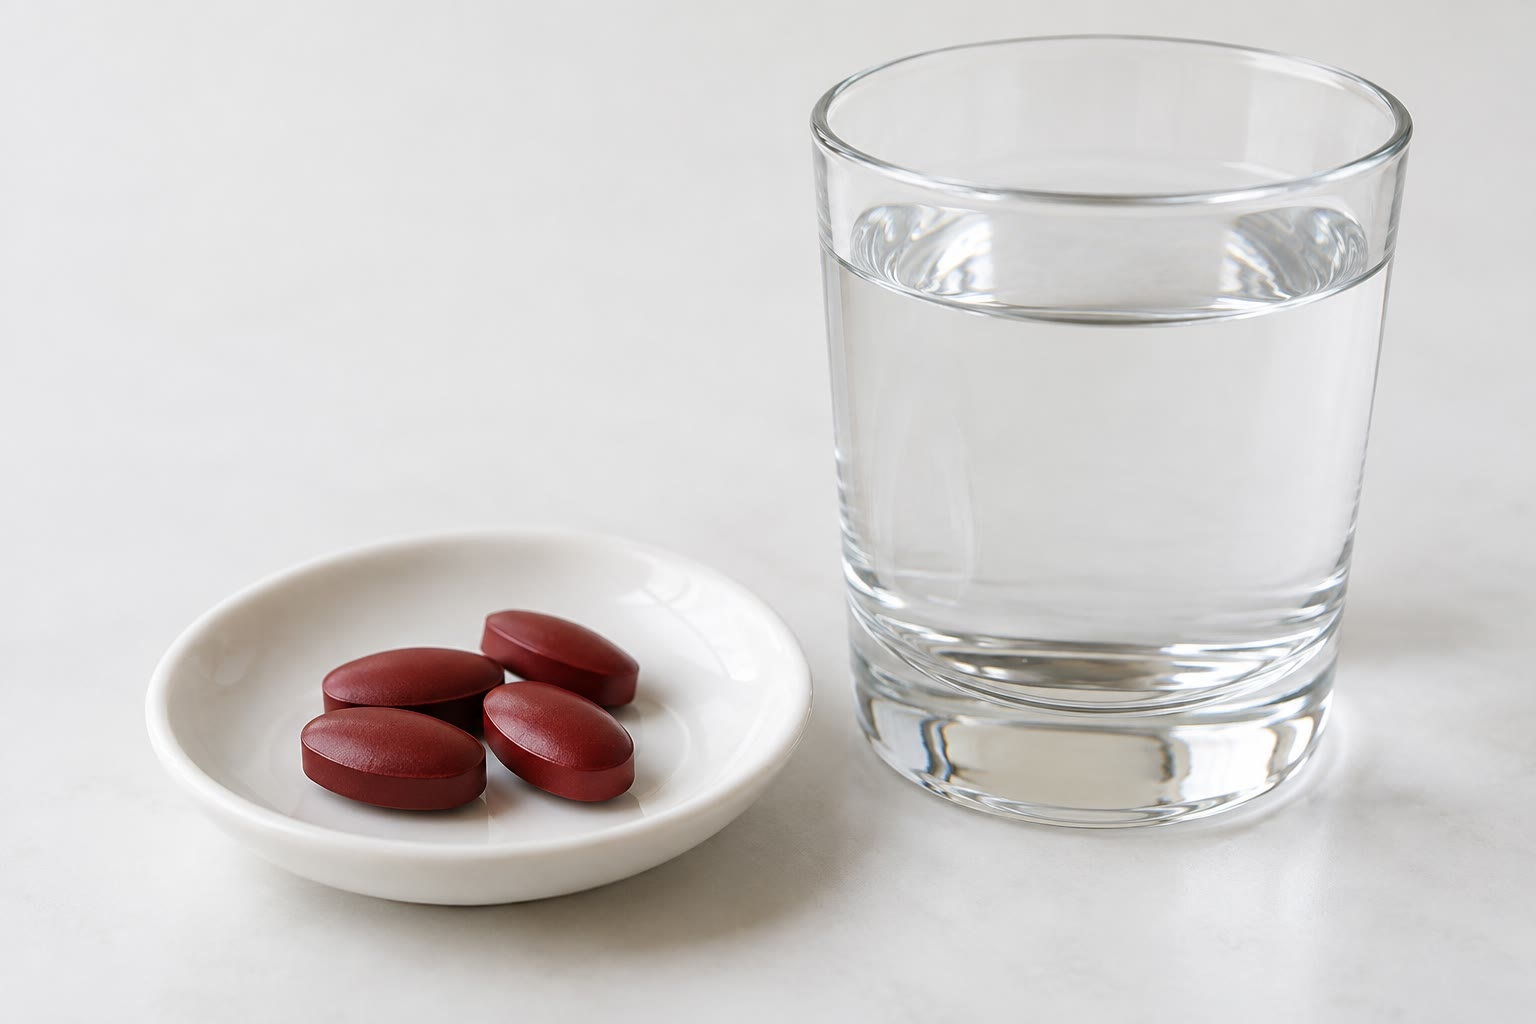
\includegraphics[width=0.45\linewidth]{images/book1/ai/g11-iron-tablets.jpg}

{\small Tabletten met een ijzersupplement: hoeveel ijzer zit er werkelijk
in elke tablet?}
\end{omfigure}

\section{Titreren}

\begin{definition}[Titratie, titrant, getitreerde oplossing]\label{def:g11:titration:titration}
Een \emph{titratie}\index{titratie} meet de hoeveelheid van een opgelost
deeltje door het te laten reageren met een ander deeltje waarvan de
concentratie nauwkeurig bekend is. De oplossing met de bekende
concentratie, die uit een buret wordt toegevoegd, is de
\emph{titrant}\index{titrant}; de oplossing met het deeltje dat gemeten
moet worden, die in de erlenmeyer staat, is de \emph{getitreerde
oplossing}\index{getitreerde oplossing}.
\end{definition}

\begin{proposition}[Waaraan een titratiereactie moet voldoen]\label{prop:g11:titration:conditions}
Een reactie is bruikbaar voor een \omterm{def:g11:titration:titration}{titratie} als ze aflopend is (zodat één
\omterm{def:g7:chemical-reactions:reactant}{beginstof} helemaal verbruikt wordt), snel (zodat elke druppel meteen
reageert) en eenduidig (de \omterm{def:g11:titration:titration}{titrant} reageert met niets anders in de
erlenmeyer).
\end{proposition}

\begin{proof}
Als de reactie stopte voordat ze af was, achterliep op de druppels of
ergens anders \omterm{def:g11:titration:titration}{titrant} verbruikte, zou het toegevoegde volume niet langer
de hoeveelheid van het getitreerde deeltje meten.
\end{proof}

\begin{omfigure}
\begin{tikzpicture}[font=\small, scale=0.62]
  \pic[transform shape] at (0,0) {stand={5.8}{1.8}};
  \pic[transform shape] at (1.8,0.68) {stirrer};
  \pic[transform shape] at (1.8,0.68) {erlenmeyer={0.25}{yellow!12}};
  \pic[transform shape] at (1.8,2.98) {burette={0.75}{violet!55}};
  \draw[omProp, thick, <-] (2.15,6.9) -- (4.2,7.4) node[right, text=black,
    align=left] {buret: titrant\\ (kaliumpermanganaat)};
  \draw[omProp, thick, <-] (2.55,1.4) -- (4.2,1.9) node[right, text=black,
    align=left] {erlenmeyer: getitreerde\\ oplossing (ijzer(II), zuur)};
  \draw[omProp, thick, <-] (3.0,0.4) -- (4.2,0.3) node[right, text=black]
    {magneetroerder};
\end{tikzpicture}

{\small Een titratieopstelling: de buret, vastgezet aan een statief, voegt
de \omterm{def:g11:titration:titration}{titrant} toe aan de \omterm{def:g11:titration:titration}{getitreerde oplossing}, die geroerd wordt.}
\end{omfigure}

\section{Het equivalentiepunt}

\begin{definition}[Equivalentiepunt, equivalentievolume]\label{def:g11:titration:equivalence}
Het \emph{equivalentiepunt}\index{equivalentiepunt} is het moment in een
\omterm{def:g11:titration:titration}{titratie} waarop de toegevoegde \omterm{def:g11:titration:titration}{titrant} en het getitreerde deeltje in de
verhouding van de \omterm{def:g8:balanced-equations:equation}{reactievergelijking} aanwezig zijn: beide zijn
verbruikt. Het volume \omterm{def:g11:titration:titration}{titrant} dat op dat moment is toegevoegd, is het
\emph{equivalentievolume}\index{equivalentievolume}, $V_E$.
\end{definition}

\begin{proposition}[Het verband bij het equivalentiepunt]\label{prop:g11:titration:relation}
Voor een titratiereactie $a\,\ce{A} + b\,\ce{B} \longrightarrow$ producten, waarin A (hoeveelheid
$n_A$) getitreerd wordt met een \omterm{def:g11:titration:titration}{titrant} B met concentratie $c_B$, geldt
bij het \omterm{def:g11:titration:equivalence}{equivalentiepunt}
\[
  \frac{n_A}{a} = \frac{c_B\, V_E}{b} .
\]
\end{proposition}

\begin{proof}
Bij het \omterm{def:g11:titration:equivalence}{equivalentiepunt} is het \omterm{def:g6:pure-substances-and-mixtures:mixture}{mengsel} stoichiometrisch
(\cref{ch:g10:reaction-progress-table}): A en B, met beginhoeveelheden $n_A$
en $c_B V_E$, raken tegelijk op, dus $n_A / a = c_B V_E / b$.
\end{proof}

\begin{omfigure}
\begin{tikzpicture}
\begin{axis}[width=0.72\linewidth, height=5.6cm, xmin=0, xmax=20,
    ymin=0, ymax=16, xlabel={toegevoegd volume titrant (\si{mL})},
    ylabel={hoeveelheid ($\num{e-4}$ \si{mol})}, axis lines*=left, ymajorgrids,
    grid style={gray!20}, tick label style={font=\small},
    label style={font=\small}, legend style={font=\small, at={(0.98,0.97)},
    anchor=north east, draw=none}, legend cell align=left]
  \addplot[very thick, orange!70!black, domain=0:14.3] {14.3 - x};
  \addplot[very thick, violet, domain=14.3:20] {0.2*(x - 14.3)};
  \addplot[very thick, violet, domain=0:14.3, forget plot] {0};
  \legend{\ce{Fe^{2+}} nog in de erlenmeyer, \ce{MnO4^-} in overmaat}
  \addplot[dashed, black!60] coordinates {(14.3,0) (14.3,7)};
  \node[font=\small, anchor=west] at (axis cs:14.5,6.5) {$V_E = \qty{14.3}{mL}$};
\end{axis}
\end{tikzpicture}

{\small IJzer(II) getitreerd met permanganaat van \qty{0.0200}{mol/L}: de
ijzer(II)\omterm{def:g9:ions:ion}{ionen} raken precies bij het \omterm{def:g11:titration:equivalence}{equivalentievolume} op; daarna worden
de permanganaationen niet meer verbruikt en hopen ze zich op.}
\end{omfigure}

\section{Het equivalentiepunt vinden aan een kleuromslag}


\begin{proposition}[Het equivalentiepunt zien]\label{prop:g11:titration:colour}
Als een van de deeltjes van de \omterm{def:g11:titration:titration}{titratie} gekleurd is, zie je het
\omterm{def:g11:titration:equivalence}{equivalentiepunt} als een kleuromslag in de erlenmeyer: de kleur van de
\omterm{def:g11:titration:titration}{titrant} verschijnt en blijft zodra de \omterm{def:g11:titration:titration}{titrant} in overmaat is, of de
kleur van het getitreerde deeltje verdwijnt wanneer dat op raakt.
\end{proposition}

\begin{proof}
Vóór het \omterm{def:g11:titration:equivalence}{equivalentiepunt} wordt elk \omterm{def:g9:ions:ion}{ion} \omterm{def:g11:titration:titration}{titrant} dat in de erlenmeyer valt
meteen verbruikt; na het \omterm{def:g11:titration:equivalence}{equivalentiepunt} blijft het over. Een gekleurd
deeltje is dus maar aan één kant van het \omterm{def:g11:titration:equivalence}{equivalentiepunt} in de
erlenmeyer aanwezig.
\end{proof}

\begin{example}[Permanganaat, zijn eigen indicator]\label{ex:g11:titration:permanganate}
Het permanganaation \ce{MnO4^-} is dieppaars, en de mangaanionen
\ce{Mn^{2+}} die het oplevert, zijn bijna kleurloos; de ijzerionen geven
de oplossing alleen een lichtgele tint. Vóór het \omterm{def:g11:titration:equivalence}{equivalentiepunt} wordt
elke paarse druppel ontkleurd zodra hij valt; de eerste druppel die niet
ontkleurt, markeert het \omterm{def:g11:titration:equivalence}{equivalentiepunt}: de erlenmeyer wordt lichtroze
en blijft dat.
\end{example}

\begin{omfigure}
\begin{tikzpicture}[font=\small]
  \pic at (0,0) {erlenmeyer={0.3}{yellow!14}};
  \pic at (3.2,0) {erlenmeyer={0.3}{magenta!10}};
  \pic at (6.4,0) {erlenmeyer={0.3}{violet!45}};
  \node[align=center, anchor=north, font=\footnotesize] at (0,-0.15) {vóór het\\
    equivalentiepunt:\\ lichtgeel, elke\\ druppel ontkleurd};
  \node[align=center, anchor=north, font=\footnotesize] at (3.2,-0.15) {bij het\\
    equivalentiepunt:\\ zwakke roze kleur\\ die blijft};
  \node[align=center, anchor=north, font=\footnotesize] at (6.4,-0.15) {na het\\
    equivalentiepunt:\\ paars (perman-\\ ganaat in overmaat)};
\end{tikzpicture}

{\small De erlenmeyer van een \omterm{def:g11:titration:titration}{titratie} van ijzer(II) met permanganaat,
vóór, bij en na het \omterm{def:g11:titration:equivalence}{equivalentiepunt}. Het \omterm{def:g11:titration:equivalence}{equivalentievolume} lees je af
bij de eerste blijvende roze kleur.}
\end{omfigure}

\begin{example}[Vitamine C en jood]\label{ex:g11:titration:vitamin-c}
% ledger: aw:C, aw:H, aw:O
Vitamine C, ascorbinezuur \ce{C6H8O6} ($M = \qty{176.0}{g/mol}$), is een
\omterm{def:g11:redox:oxidant}{reductor}; jood \ce{I2} oxideert het:
\[
  \ce{C6H8O6 + I2 -> C6H6O6 + 2H+ + 2I-} .
\]
\qty{10.0}{mL} sinaasappelsap, met een beetje zetmeel, wordt getitreerd
met een joodoplossing van \qty{5.00e-3}{mol/L}. Vóór het
\omterm{def:g11:titration:equivalence}{equivalentiepunt} wordt het jood verbruikt; de eerste druppel in overmaat
kleurt het zetmeel donkerblauw. Als
$V_E = \qty{5.70}{mL}$, bevatte het sap
$n = \num{5.00e-3} \times \num{5.70e-3} = \qty{2.85e-5}{mol}$ vitamine
C, dat is \qty{5.0}{mg} in \qty{10.0}{mL}: \qty{0.50}{g/L}.
\end{example}

\section{Een onbekende concentratie berekenen}

\begin{method}[Een concentratie berekenen uit een titratie]\label{met:g11:titration:computing}
\begin{enumerate}
  \item Schrijf de \omterm{def:g8:balanced-equations:equation}{kloppende reactievergelijking} van de titratiereactie
        op en lees de \omterm{def:g8:balanced-equations:coefficient}{coëfficiënten} $a$ (getitreerd deeltje) en $b$
        (\omterm{def:g11:titration:titration}{titrant}) af.
  \item Lees $V_E$ af op de buret, en bereken de hoeveelheid toegevoegde
        \omterm{def:g11:titration:titration}{titrant}, $n_B = c_B V_E$.
  \item Bij het \omterm{def:g11:titration:equivalence}{equivalentiepunt} geldt $n_A = \dfrac{a}{b}\, c_B V_E$.
  \item Deel door het getitreerde volume: $c_A = n_A / V_A$. Als het
        monster vóór de \omterm{def:g11:titration:titration}{titratie} verdund is, vermenigvuldig dan met de
        \omterm{def:g10:concentration-and-dilution:dilution}{verdunningsfactor}.
\end{enumerate}
\end{method}

\begin{example}[Een ijzer(II)oplossing]\label{ex:g11:titration:iron}
Voor \qty{20.0}{mL} van een aangezuurde ijzer(II)oplossing is
$V_E = \qty{12.6}{mL}$ permanganaat van \qty{0.0200}{mol/L} nodig. Hier
$a = 5$ (\ce{Fe^{2+}}) en $b = 1$ (\ce{MnO4^-}):
$n(\ce{MnO4^-}) = 0.0200 \times 0.0126 = \qty{2.52e-4}{mol}$, dus
$n(\ce{Fe^{2+}}) = 5 \times \num{2.52e-4} = \qty{1.26e-3}{mol}$, en
$c(\ce{Fe^{2+}}) = \num{1.26e-3} / 0.0200 = \qty{0.0630}{mol/L}$.
\end{example}

\section{De titratie als meting}

\begin{inthelab}[Een buret aflezen]
De buret wordt omgespoeld met de \omterm{def:g11:titration:titration}{titrant}, gevuld, en de punt wordt vrij
gemaakt van luchtbellen. Het niveau lees je af aan de onderkant van de
meniscus, met je oog op dezelfde hoogte, vóór en na de \omterm{def:g11:titration:titration}{titratie}: het
toegevoegde volume is het verschil. De maatstreepjes staan om de
\qty{0.1}{mL}, en een aflezing kun je schatten tot op \qty{0.05}{mL}.
Vlak bij het \omterm{def:g11:titration:equivalence}{equivalentiepunt} wordt de \omterm{def:g11:titration:titration}{titrant} druppel voor druppel
toegevoegd, terwijl de erlenmeyer gezwenkt of geroerd wordt.
\end{inthelab}

\begin{omfigure}
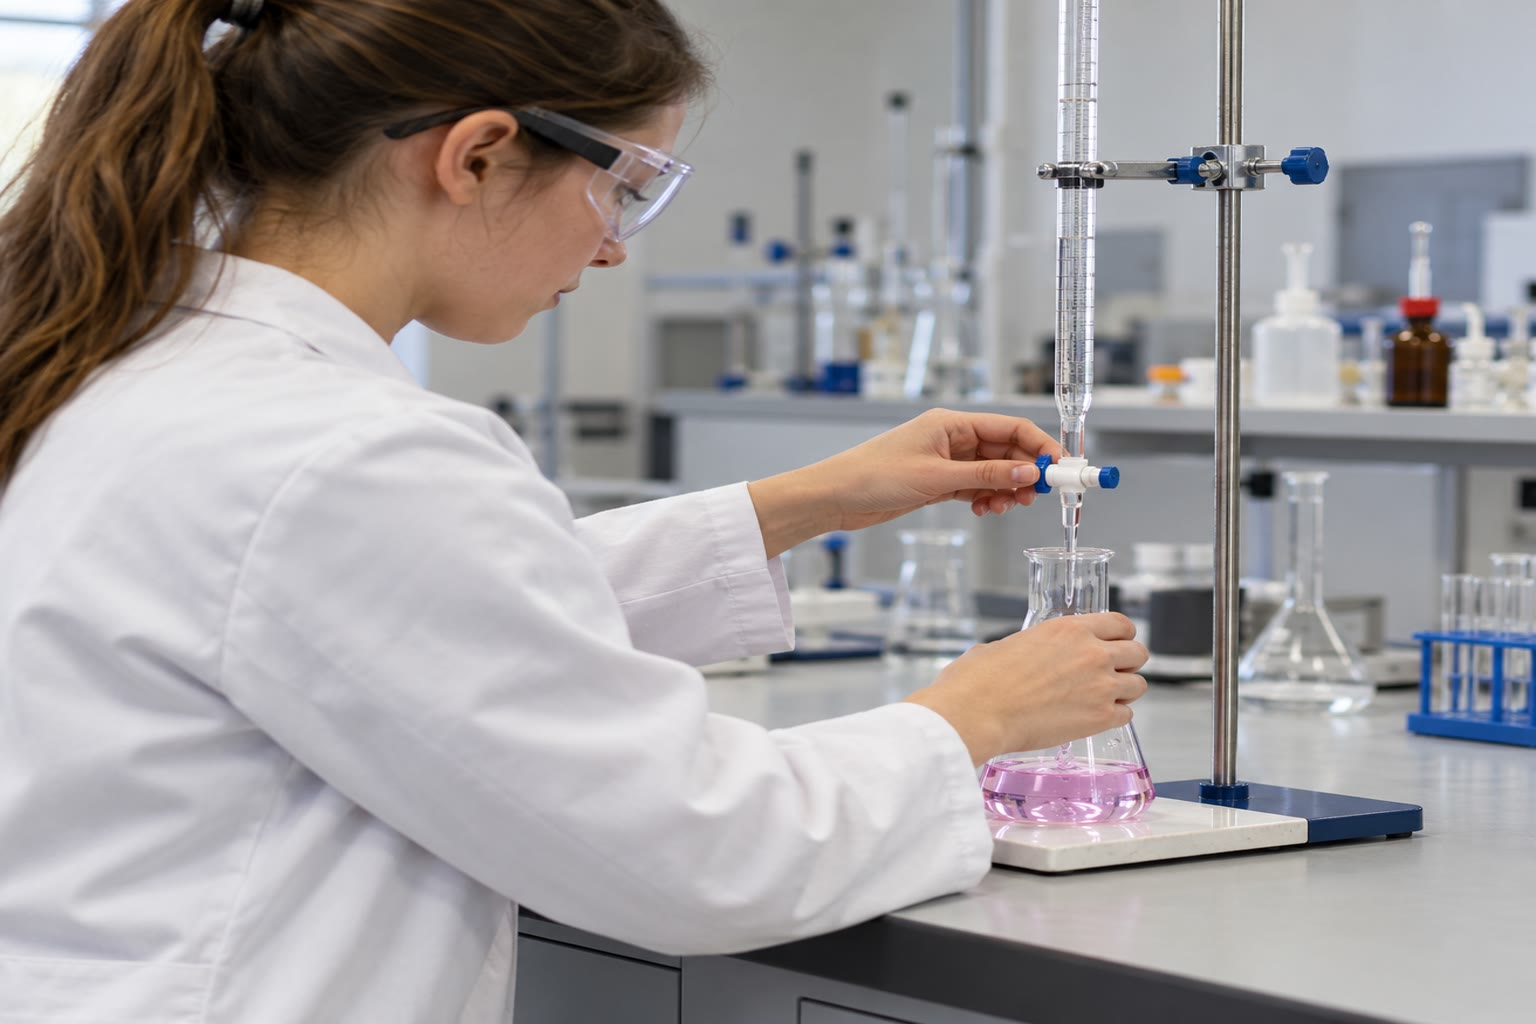
\includegraphics[width=0.48\linewidth]{images/book1/ai/g11-titration-bench.jpg}

{\small Een \omterm{def:g11:titration:titration}{titratie} in uitvoering: buret, statief en erlenmeyer op een
witte tegel.}
\end{omfigure}

\begin{remark}[Hoe nauwkeurig is een titratie?]\label{rem:g11:titration:precision}
Elke aflezing van de buret kan er ongeveer \qty{0.05}{mL} naast zitten,
en het toegevoegde volume is het verschil van twee aflezingen: dat kan
er dus tot \qty{0.1}{mL} naast zitten. Voor $V_E = \qty{14.3}{mL}$ is dat
$0.1 / 14.3 \approx
\qty{0.7}{\percent}$. Een groter $V_E$ maakt deze relatieve fout
kleiner; daarom kiest men de concentratie van de \omterm{def:g11:titration:titration}{titrant} zo dat het
\omterm{def:g11:titration:equivalence}{equivalentievolume} tussen 10 en \qty{20}{mL} ligt bij een buret van
\qty{25}{mL}. De \omterm{def:g11:titration:titration}{titratie} wordt herhaald tot twee resultaten tot op
ongeveer \qty{0.1}{mL} overeenkomen. Een preciezere behandeling van de
onzekerheid van een meting volgt in het deel voor het eerste
universiteitsjaar.
\end{remark}

\begin{safety}{\ghs[0.7cm]{GHS03}\ghs[0.7cm]{GHS05}\ghs[0.7cm]{GHS07}\ghs[0.7cm]{GHS08}\ghs[0.7cm]{GHS09}}
% ledger: ghs:KMnO4, ghs:I2
Vast kaliumpermanganaat is een \omterm{def:g11:redox:oxidant}{oxidator} die een brand kan aanwakkeren,
bijtend en schadelijk; verdunde oplossingen ervan kleuren huid en kleding
bruin. Joodoplossingen zijn schadelijk. Veiligheidsbril en handschoenen;
het afval wordt ingezameld en gaat nooit door de gootsteen.
\end{safety}

\section{Oefeningen}


\begin{exercise}[$\star$]\label{exo:g11:titration:1}
Wat is bij een \omterm{def:g11:titration:titration}{titratie} de \omterm{def:g11:titration:titration}{titrant}? En de \omterm{def:g11:titration:titration}{getitreerde oplossing}? Wat
gebeurt er bij het \omterm{def:g11:titration:equivalence}{equivalentiepunt}?
\end{exercise}

\begin{exercise}[$\star$]\label{exo:g11:titration:2}
Welke hoeveelheid permanganaationen zit er in \qty{12.5}{mL} van een
oplossing van \qty{0.0200}{mol/L}?
\end{exercise}

\begin{exercise}[$\star$]\label{exo:g11:titration:3}
Lees in de figuur van de hoeveelheden tegen het toegevoegde volume het
\omterm{def:g11:titration:equivalence}{equivalentievolume} af. Welke hoeveelheid ijzer(II) zat er aan het begin
in de erlenmeyer?
\end{exercise}

\begin{exercise}[$\star$]\label{exo:g11:titration:4}
Waarom is er bij een \omterm{def:g11:titration:titration}{titratie} met permanganaat geen indicator nodig?
\end{exercise}

\begin{exercise}[$\star$]\label{exo:g11:titration:5}
Wat is bij het \omterm{def:g11:titration:equivalence}{equivalentiepunt} van de \omterm{def:g11:titration:titration}{titratie} van ijzer(II) met
permanganaat de verhouding tussen de hoeveelheid ijzer(II) en de
hoeveelheid toegevoegd permanganaat? Waarom?
\end{exercise}

\begin{exercise}[$\star\star$]\label{exo:g11:titration:6}
Voor \qty{10.0}{mL} van een aangezuurde ijzer(II)oplossing is
\qty{8.40}{mL} permanganaat van \qty{0.0200}{mol/L} nodig. Bereken de
\omterm{def:g10:concentration-and-dilution:molar-concentration}{molaire concentratie} van ijzer(II), en daarna de \omterm{def:g10:concentration-and-dilution:mass-concentration}{massaconcentratie}.
\end{exercise}

\begin{exercise}[$\star\star$]\label{exo:g11:titration:7}
Een vitamine C-tablet wordt opgelost tot \qty{100.0}{mL} oplossing.
Voor \qty{10.0}{mL} daarvan, met zetmeel, is \qty{11.4}{mL} jood van
\qty{0.0100}{mol/L} nodig. Welke massa vitamine C bevat de tablet?
\end{exercise}

\begin{exercise}[$\star\star$]\label{exo:g11:titration:8}
Een reactie is aflopend, maar duurt een paar minuten. Waarom kun je haar
niet zomaar gebruiken voor een \omterm{def:g11:titration:titration}{titratie} met een kleuromslag?
\end{exercise}

\begin{exercise}[$\star\star$]\label{exo:g11:titration:9}
Bekijk de drie erlenmeyers. Een leerling stopt bij een erlenmeyer die
even paars is als de derde. Is haar \omterm{def:g11:titration:equivalence}{equivalentievolume} te groot of te
klein? Wat had ze vlak bij het \omterm{def:g11:titration:equivalence}{equivalentiepunt} moeten doen?
\end{exercise}

\begin{exercise}[$\star\star$]\label{exo:g11:titration:10}
Een geconcentreerde ijzer(II)oplossing wordt eerst tien keer verdund.
Daarna is voor \qty{10.0}{mL} van de verdunde oplossing \qty{13.0}{mL}
permanganaat van \qty{0.0200}{mol/L} nodig. Bereken de concentratie van
de geconcentreerde oplossing.
\end{exercise}

\begin{exercise}[$\star\star$]\label{exo:g11:titration:11}
% ledger: aw:Fe
De ijzer(II)oplossing uit het uitgewerkte voorbeeld van dit hoofdstuk
heeft $c = \qty{0.0630}{mol/L}$. Welke massa ijzer bevat \qty{1.00}{L}
ervan?
\end{exercise}

\begin{exercise}[$\star\star\star$]\label{exo:g11:titration:12}
Een \omterm{def:g11:titration:titration}{titratie} geeft $V_E = \qty{7.2}{mL}$. Schat de relatieve fout door
de aflezingen van de buret, en vergelijk met $V_E = \qty{14.3}{mL}$.
Bedenk twee manieren om een groter \omterm{def:g11:titration:equivalence}{equivalentievolume} te krijgen.
\end{exercise}

\begin{exercise}[$\star\star\star$]\label{exo:g11:titration:13}
Waterstofperoxide wordt in zuur milieu getitreerd met permanganaat:
\[
  \ce{2MnO4^- + 5H2O2 + 6H+ -> 2Mn^{2+} + 5O2 + 8H2O} .
\]
Een ontsmettingsmiddel wordt tien keer verdund; voor \qty{10.0}{mL} van
de verdunde oplossing is \qty{17.6}{mL} permanganaat van
\qty{0.0200}{mol/L} nodig. Bereken de \omterm{def:g10:concentration-and-dilution:molar-concentration}{molaire concentratie} van
waterstofperoxide in het ontsmettingsmiddel, en daarna de
\omterm{def:g10:concentration-and-dilution:mass-concentration}{massaconcentratie} (\ce{H2O2}: \qty{34.0}{g/mol}).
\end{exercise}

\begin{exercise}[$\star\star\star$]\label{exo:g11:titration:14}
Een ijzertablet hoort ongeveer \qty{1.4e-3}{mol} ijzer(II) te bevatten.
Welke concentratie permanganaat geeft een \omterm{def:g11:titration:equivalence}{equivalentievolume} van
ongeveer \qty{15}{mL} bij een buret van \qty{25}{mL}? Wat zou er
misgaan met een oplossing die tien keer zo geconcentreerd is?
\end{exercise}

\begin{exercise}[$\star\star\star$]\label{exo:g11:titration:15}
De vergelijking van de \omterm{def:g11:titration:titration}{titratie} bevat \ce{8H+} per \ce{MnO4^-}. Welke
hoeveelheid waterstofionen wordt er verbruikt bij een \omterm{def:g11:titration:equivalence}{equivalentievolume}
van \qty{14.3}{mL} van \qty{0.0200}{mol/L}? Is \qty{10}{mL} van een zuur
met \qty{1.0}{mol/L} waterstofionen genoeg? Waarom moet de erlenmeyer
aangezuurd worden?
\end{exercise}

\section{Probleem: Is de ijzertablet eerlijk?}

\begin{problem}[{Weekendprobleem --- een ijzersupplement belooft 80 mg
ijzer per tablet: is een titratie het daarmee eens?}]
\label{pb:g11:titration:1}
% ledger: aw:Fe, aw:S, aw:O, const:NA
Op het doosje van een ijzersupplement staat \qty{80}{mg} ijzer, als
ijzer(II), per tablet. Een tablet wordt verpulverd en opgelost in
ongeveer \qty{50}{mL} verdund zwavelzuur, en daarna getitreerd met
kaliumpermanganaat van \qty{0.0200}{mol/L}. De zwakke roze kleur blijft
bij $V_E = \qty{14.3}{mL}$.

\medskip
\noindent\textbf{Deel I --- De reactie.}
\begin{enumerate}
  \item Noem de twee \omterm{def:g11:redox:couple}{redoxkoppels} die meedoen. Welk deeltje is de
        \omterm{def:g11:redox:oxidant}{oxidator}, welk de \omterm{def:g11:redox:oxidant}{reductor}?
  \item Schrijf de twee \omterm{def:g11:redox:couple}{halfreacties} op.
  \item Combineer ze tot de vergelijking van de \omterm{def:g11:titration:titration}{titratie}, en controleer
        dat de lading klopt.
  \item Waarom wordt de tablet in zuur opgelost?
  \item Laat zien dat de reactie voldoet aan de voorwaarden voor een
        \omterm{def:g11:titration:titration}{titratie}, en leg uit hoe je het \omterm{def:g11:titration:equivalence}{equivalentiepunt} ziet.
\end{enumerate}

\medskip
\noindent\textbf{Deel II --- De \omterm{def:g11:titration:titration}{titratie}.}
\begin{enumerate}[resume]
  \item In welk glaswerk zit de permanganaatoplossing? Hoe lees je het
        volume ervan af?
  \item Welke kleur heeft de erlenmeyer vóór het \omterm{def:g11:titration:equivalence}{equivalentiepunt}, en
        waarom verliest elke druppel zijn kleur?
  \item Bereken de hoeveelheid permanganaat die bij het \omterm{def:g11:titration:equivalence}{equivalentiepunt}
        is toegevoegd.
\end{enumerate}

\medskip
\noindent\textbf{Deel III --- Het ijzer.}
\begin{enumerate}[resume]
  \item Leid de hoeveelheid ijzer(II) in de tablet af.
  \item Bereken de massa ervan in milligram.
  \item Vergelijk met het etiket: wat is het relatieve verschil?
  \item Het toegevoegde volume kan er \qty{0.1}{mL} naast zitten. Hoeveel
        milligram kan de massa ijzer ernaast zitten? Wordt het etiket
        bevestigd?
\end{enumerate}

\medskip
\noindent\textbf{Deel IV --- Meer tabletten.}
\begin{enumerate}[resume]
  \item Twee andere tabletten geven $V_E = \qty{14.1}{mL}$ en
        \qty{14.4}{mL}. Bereken hun massa's ijzer.
  \item Bereken het gemiddelde van de drie tabletten.
  \item De drie resultaten verschillen meer dan de fout van de buret.
        Wat zegt dat over de tabletten?
  \item Was permanganaat van \qty{0.100}{mol/L} een betere keuze geweest?
        Leg uit.
  \item Veel supplementen bevatten ook vitamine C, een \omterm{def:g11:redox:oxidant}{reductor}. Wat zou
        die doen met de \omterm{def:g11:titration:titration}{titratie}, en met de gevonden massa ijzer?
  \item Het ijzer is aanwezig als ijzer(II)sulfaat, \ce{FeSO4}. Welke
        massa daarvan bevat één tablet?
  \item Hoeveel ijzer(II)\omterm{def:g9:ions:ion}{ionen} zijn dat?
  \item Geef het eindantwoord: welke massa ijzer bevat één tablet?
\end{enumerate}
\end{problem}
